\begin{figure}[t]
    \subfigure[Impact of Proxy Model Size]{
    \begin{minipage}[t]{0.45\linewidth}
        \centering
        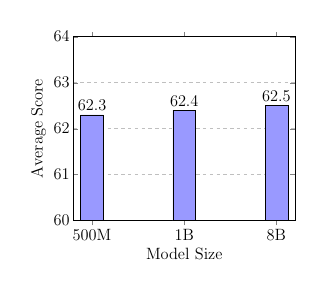
\begin{tikzpicture}[scale=0.41]
        \begin{axis}[
            xlabel={Model Size},
            ylabel={Average Score},
            symbolic x coords={500M,1B,8B},
            xtick=data,
            ymajorgrids=true,
            grid style=dashed,
            ymin=60,
            ymax=64,
            ybar,
            bar width=20pt,
            font=\Large,
            nodes near coords,
            nodes near coords align={vertical},
        ]
        \addplot[fill=blue!40] coordinates {
            (500M,62.3)
            (1B,62.4)
            (8B,62.5)
        };
        \end{axis}
        \end{tikzpicture}
    \end{minipage}
    }%
    \subfigure[Impact of Domain Count]{
    \begin{minipage}[t]{0.45\linewidth}
        \centering
        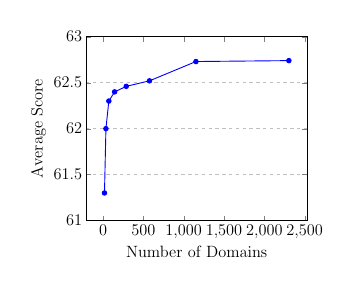
\begin{tikzpicture}[scale=0.41]
        \begin{axis}[
            xlabel={Number of Domains},
            ylabel={Average Score},
            legend style={at={(0.98,0.02)}, anchor=south east},
            ymajorgrids=true,
            grid style=dashed,
            ymin=61,
            ymax=63,
            % xtick={18,36,72,144,288,576,1152},
            font=\Large,
            % mark options={scale=1.5}
        ]
        \addplot[thick,mark=*,blue] coordinates {
            (18,61.3)
            (36,62.0)
            (72,62.3)
            (144,62.4)
            (288,62.46)
            (576,62.52)
            (1152,62.73)
            (2304,62.74)
        };
        \end{axis}
        \end{tikzpicture}
    \end{minipage}
    }
    \vspace{-0.3cm}
    \caption{Effects of model size and domain count.}
    \label{fig:model-analysis}
    \vspace{-0.5cm}
\end{figure}